\documentclass[10pt,oneside]{article}
\usepackage{amsmath} % Refined math symbols
%Declare new operator
\DeclareMathOperator{\proj}{Proj}
\usepackage{graphicx} % Images
\usepackage{subcaption} % The hability of using subfigures
\usepackage{amsfonts}
\usepackage{amssymb} % To use the symbols for numerical sets

% Language options (we set two languages in this text)
\usepackage{polyglossia}
\setmainlanguage[variant=american]{english}
\setotherlanguage{spanish}

% New bibliography system: biber (No bibtex needed)
\usepackage[
  backend=biber
]{biblatex}
\addbibresource{biblio.bib}

%Set the margins and papersize
\usepackage[
  letterpaper,
  left=1cm,
  right=1cm,
  top=1.5cm,
  bottom=1.5cm
]{geometry}

% custom links and pdf metadata
\usepackage[
  final,
  unicode,
  colorlinks=true,
  citecolor=blue,
  linkcolor=blue,
  plainpages=false,
  urlcolor=blue,
  pdfpagelabels=true,
  pdfsubject={Study Notes for Coding Interview},
  pdfauthor={Jorge Antonio García Galicia},
  pdftitle={StudyNotes},
  pdfkeywords={Google, Nvidia, code, interview, codding}
]{hyperref}

%Profesionall looking tables
\usepackage{booktabs}

%To insert algorithms in pseudocode
\usepackage{algpseudocode}
\usepackage{algorithm} %float enviroment for algorithms
%Make the comments similar to cpp
%\algrenewcommand{\algorithmiccomment}[1]{\hskip3em$//$ #1}

%Headers and footers
\usepackage{lastpage}
\usepackage{fancyhdr}
\fancyhf{}
\pagestyle{fancy}
\fancyhf{}
\fancyhead[L]{Study Notes for Coding Interview}
\fancyhead[C]{Jorge Antonio Garc\'ia Galicia} %There is no utf8 in fancyhdr
\fancyhead[R]{\href{mailto:nemediano@gmail.com}{nemediano@gmail.com}}
% https://tex.stackexchange.com/questions/227/how-can-i-add-page-of-on-my-document
\fancyfoot[C]{\thepage\ of \pageref*{LastPage}}
%\fancyfoot[C]{ of }
\renewcommand{\headrulewidth}{2pt} 
\renewcommand{\footrulewidth}{2pt}

\setlength{\parindent}{1em}
\setlength{\parskip}{1em}

\usepackage{minted} %For inserting source code and embed source files
%Requieres compilation using:
% $xelatex -shell-escape input.tex

%In order to work this temple needs to be build like this:
% 1 XeLaTeX
% 2 Biber 
%    This tool is not in the default Kile: I need to install the package and then configure 
%    here: https://tex.stackexchange.com/questions/154751/biblatex-with-biber-configuring-my-editor-to-avoid-undefined-citations/154763#154763)
% 3 XeLaTex
% 4 XeLateX
% 5 ViewPDF

\author{Jorge Antonio Garc\'ia Galicia} % Again, no utf8 I do not know why
\title{Study Notes}
\date{\today}

\usepackage{csquotes} % Because if this is not present HERE polyglossia throws a warning

\begin{document}
\maketitle
\thispagestyle{fancy} %So, the title page has fancyheders
\section{Memory flatenig}

A common design problem in multidimensional data situations is memory layout representation.
Internally, computers always represent memory in a linear fashion, the idea of \emph{mutidimensional array} it's just sugar syntax added by high level programming lenguajes.

\subsection{One dimensional array}

Having said that, sometimes allocations for such constructs can become dificult to use or declare by themselves.
Specially, in C++.
Lets see an example:

\begin{listing}[H]
  \inputminted[
    firstline=15, %If you omit this two fields, the whole file is pulled
    lastline=21
  ]{cpp}{src/ArrayDimensions.cpp}
  \caption{One dimensioal array (by means of \mintinline{cpp}{std::vector} class) used}
  \label{lst:1Dexample}
\end{listing}

So far, everything looks good, the sintax is clear, braket operator is helping us.
Conceptually, we have a series of variables with the same type that live in a contiguos space in memory.
See Figure~\ref{fig:1D}.

\begin{figure}[htp]
  \centering
  \begin{subfigure}[b]{0.35\textwidth}
    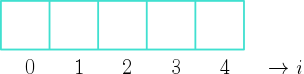
\includegraphics[width=\textwidth]{img/array1D}
    \caption{Logical memory layout representation.}
  \label{fig:1a}
  \end{subfigure}
  \hspace*{4cm}
  \begin{subfigure}[b]{0.25\textwidth}
    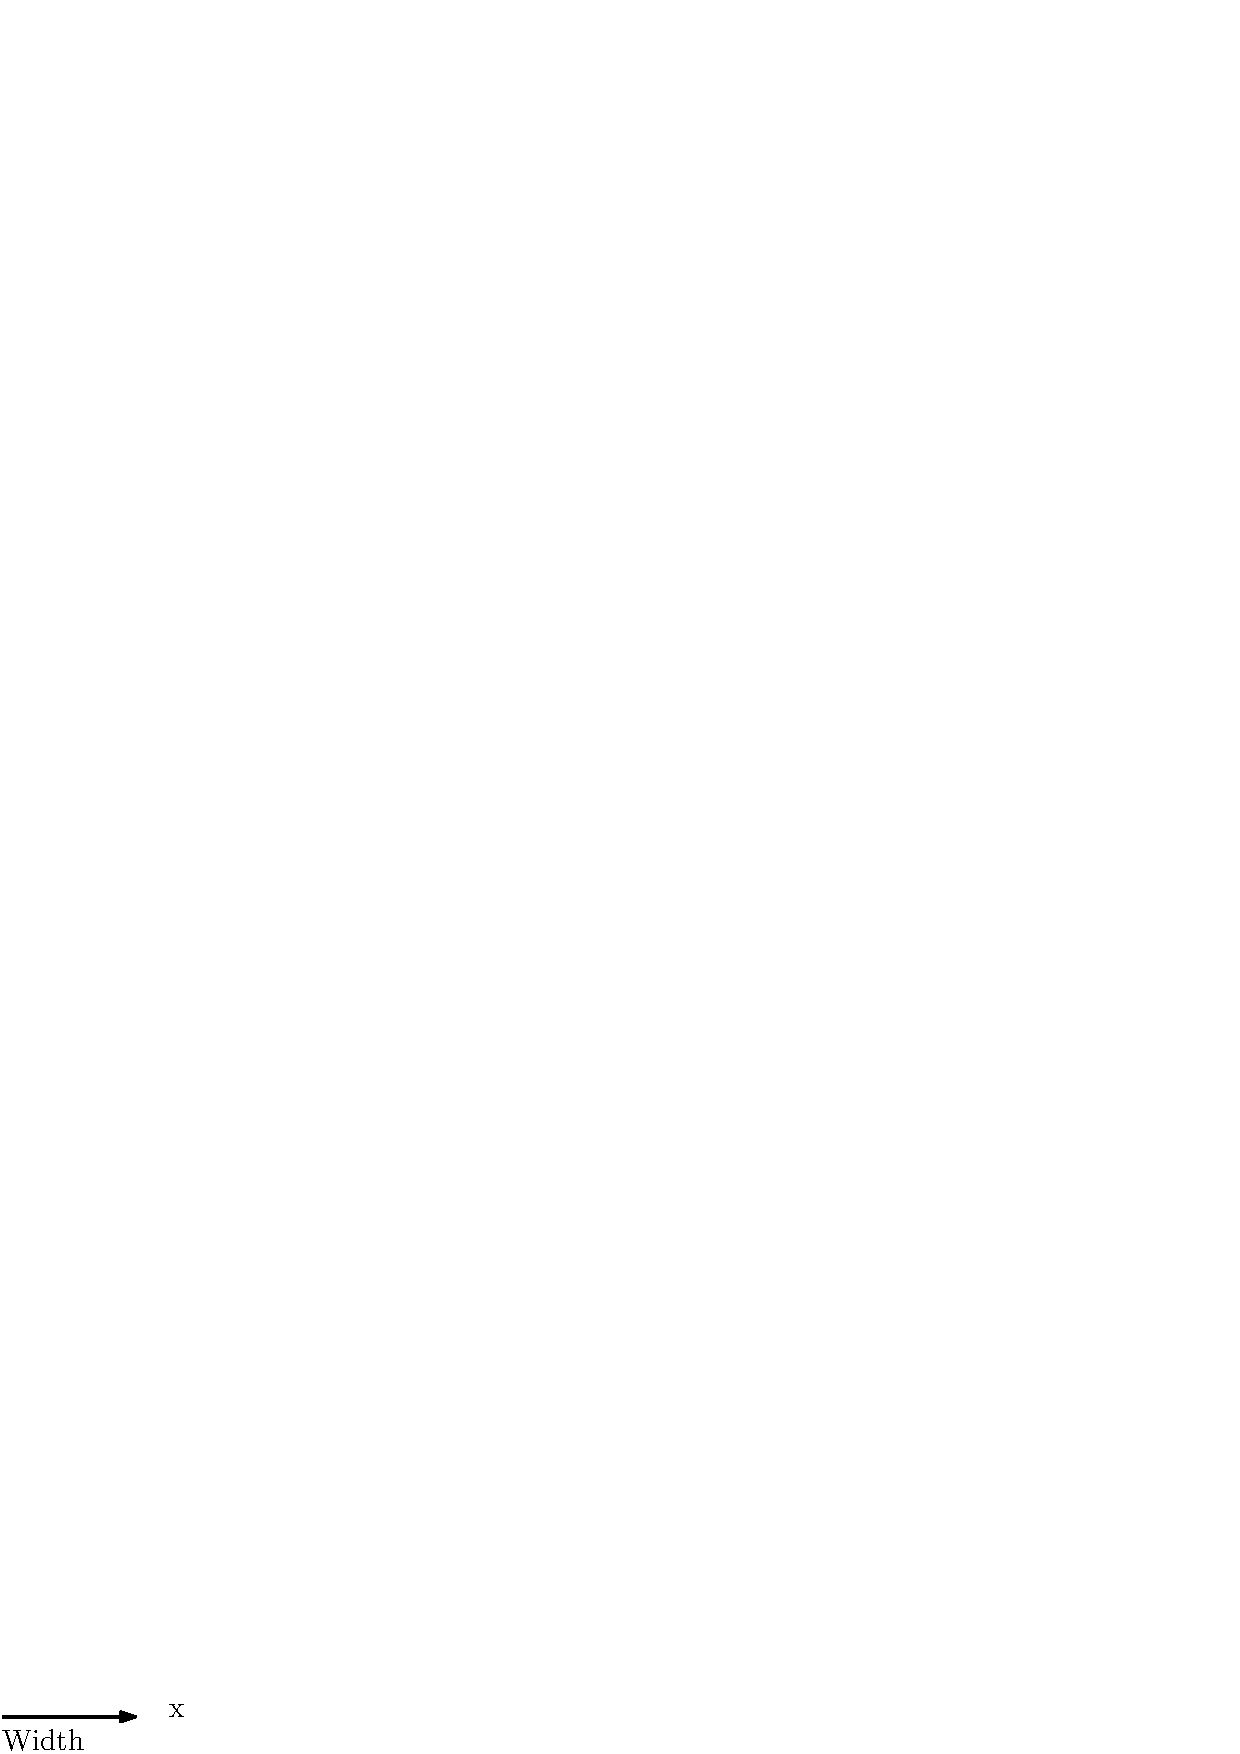
\includegraphics[width=\textwidth]{img/arrow1D}
    \caption{Dimensions represented.}
    \label{fig:1b}
  \end{subfigure}
  \caption{One dimensional array representation.}
  \label{fig:1D}
\end{figure}

\subsection{Two dimensional data}

The problem becomes evident as data start to include more dimensions.
In a bidimensional array we have data that has two dimensions.
One can think about it, like the data it's stored in a table, the situation is the one depicted in Figure~\ref{fig:2a}.
Now, remember this is just an abstraction; provided by our programming language: C++, in this case, since memory is actually \emph{close} to linear in a computer.

\begin{figure}[htp]
  \centering
  \begin{subfigure}[b]{0.35\textwidth}
    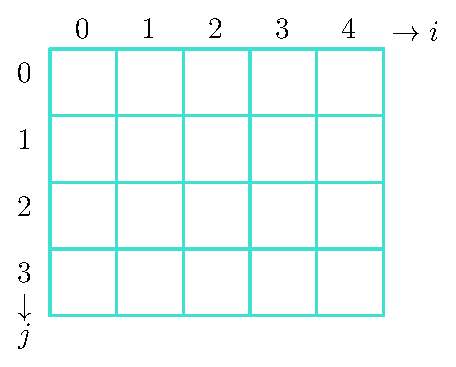
\includegraphics[width=\textwidth]{img/array2D}
    \caption{Logical memory layout representation.}
  \label{fig:2a}
  \end{subfigure}
  \hspace*{4cm}
  \begin{subfigure}[b]{0.25\textwidth}
    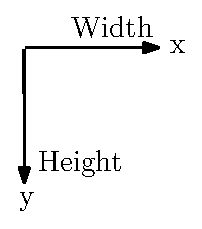
\includegraphics[width=\textwidth]{img/arrow2D}
    \caption{Dimensions represented.}
    \label{fig:2b}
  \end{subfigure}
  \caption{Two dimensional array representation.}
  \label{fig:2D}
\end{figure}

Usually, the C++ way of modeling this is creating an array, such that each element of it, is also an array.
See the code in Listing~\ref{lst:2dexample}

\begin{listing}[H]
  \inputminted[
    firstline=23, %If you omit this two fields, the whole file is pulled
    lastline=38
  ]{cpp}{src/ArrayDimensions.cpp}
  \caption{Two dimensioal array example}
  \label{lst:2dexample}
\end{listing}

Now, there is three main points to highlight in the sample:
\begin{enumerate}

\item The type of the array has change.
      Now is \emph{a vector of int vectors}.
      This led us to have a longer initialization for it too.
      Imagine that you create functions to receive or return such arrays.
      The sintax to declare the parameters will become difficult.

\item We still have the advantage of a very elegant sintax to use the array: \mintinline{cpp}{b[j][i]} give us the element on column $i$ of row $j$.

\item The sintax is backwads with respect to mathematic notation.
      See Figure~\ref{fig:2D} again.
      The index \mintinline{cpp}{i} is transversin along the $x$ dimension and the index \mintinline{cpp}{j} along the $y$ dimension.
      Therefore, the element \mintinline{cpp}{b[j][i]} it's analogous to $b(x_i, y_j)$ in math.
 \end{enumerate}

\subsection{Memory flatenig explained}

Here is when the technique called \emph{memory flattening} becomes useful.
In simple words: This is to mimic what the compiler is doing for us: use linear data.
But at the same time you also provide an abstraction, so you can access it in a similar fashion that if your data had more dimensions.
In other works you simulate the access via indices for all the required dimensions.

See the Figure~\ref{fig:Flat}.
The data is equivalent to the one shown in Figure~\ref{fig:2D} in the sense that represents a two dimensional table, whose first dimension $x$ (number of columns: $5$), is indexed by $i \in \{0, 1, 2, 3, 4\}$ and whose second dimension $y$ (number of rows: $4$) is indexed by $j \in \{0, 1, 2, 3\}$.
However, the data is stored in a one dimensional array of size $5 \cdot 4 = 20$.
The actual indices of the array $ \in \{ 0, 1, \ldots, 19 \}$ and are shown on the bottom of of Figure~\ref{fig:Flat}.
However, we also provide an abstraction to access this data via simulated indices \mintinline{cpp}{[j][i]} shown in the top of Figure~\ref{fig:Flat}

\begin{figure}[htb]
  \centering
  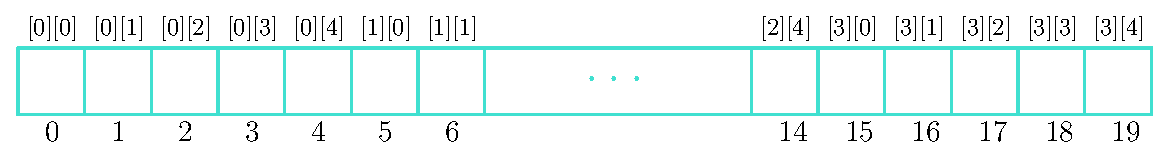
\includegraphics[width=0.85\textwidth]{img/arrayFlat}
  \caption{2D array represented as a \emph{flattened} array. This represents the same data as Figure~\ref{fig:2D}. Order of the indices is \mintinline{cpp}{[j][i]}}
  \label{fig:Flat}
\end{figure}

This has the advantage that all the data is store in a one dimensional array.
Therefore, you \emph{ensure} all your data is actually contigous in memory.
And no matter how many dimensions your data has, the type it's always a one dimensional array.

Also, provided that we acces the data in the \emph{correct way}, the access tends to be faster than the alternative shown in Listing~\ref{lst:2dexample}.
The \emph{correct way} means that the inner loop moves along the $x$ dimension and the outer loop transverses the second dimension $y$.
The reason for this improvement becomes evident if we see Figure~\ref{fig:Flat} again: in this way, we are actually accesing a linear array in his natural linear order.

In order to implement this technique we will need two mappings:
First, a function $g:\mathbb{Z}^n \rightarrow \mathbb{Z}$, to map the indices in $n$ dimensions to the one dimensional array.
And second, the inverse mapping $h:\mathbb{Z} \rightarrow \mathbb{Z}^n$ to retrive the indices back given a position in the data buffer.

The first function $g$ it is actually the most useful to us, since it will provide with the interface of accesing our data.
See the Figure~\ref{fig:2D}.
Assume that our data hast two dimensions ($x$ and $y$ --or \emph{width} and \emph{height}-- if you like).
That we use two indices $i$ and $j$ to transverse it.
And assume also that the number of cells along those dimensions are \mintinline{cpp}{WIDTH} and \mintinline{cpp}{HEIGHT} and that the indices are zero based.
In Listing~\ref{lst:functions2D} we show the implementation of such function.

We can see that the transformations are actually very simple.
In fact, one of them is the integer division and the other one is the modulo.
Also note, that as long as we check for the boundaries of the values for both indices, only one of the sizes in this case \emph{witdh} is used in the actual calculation of the indices.

\begin{listing}[H]
  \inputminted[
    firstline=88, %If you omit this two fields, the whole file is pulled
    lastline=105
  ]{cpp}{src/FlatMemmory.cpp}
  \caption{Function $g$ to map real index into simulated 2D indices}
  \label{lst:functions2D}
\end{listing}

For completeness, we also show Listing~\ref{lst:functions2D2} that defines the inverse function $h$, to retrive the index in the one dimensional array from the two simulated indices in 2D.

\begin{listing}[H]
  \inputminted[
  firstline=107, %If you omit this two fields, the whole file is pulled
  lastline=121
  ]{cpp}{src/FlatMemmory.cpp}
  \caption{Function $h$ to map simulated 2D indices into the real index, this is the inverse of $g$}
  \label{lst:functions2D2}
\end{listing}

\subsection{Three dimensional data}

Now, lets look at the more complex --but still very common-- scenario of three dimensions.
The situation is the one depicted in Figure~\ref{fig:3D}.
We include a new dimension in the data: indexed by $k$ along the $z$ axis, we call it \emph{depth}.
Note that even when the frame of reference in Figure~\ref{fig:3b}, looks weird; it is a \emph{right handed} frame of reference. 

\begin{figure}[htp]
  \centering
  \begin{subfigure}[b]{0.35\textwidth}
    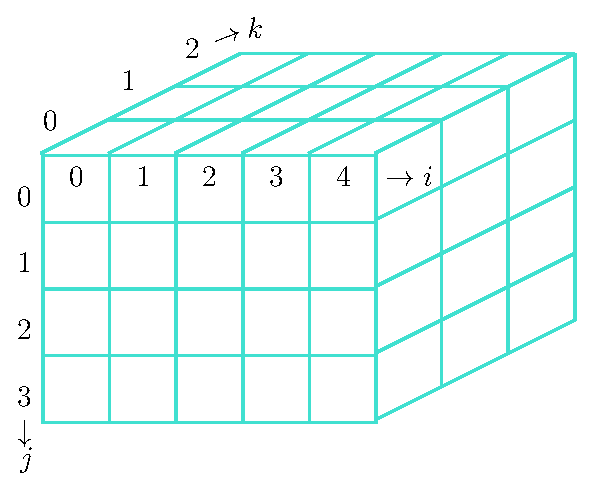
\includegraphics[width=\textwidth]{img/array3D}
    \caption{Logical memory layout representation.}
  \label{fig:3a}
  \end{subfigure}
  \hspace*{4cm}
  \begin{subfigure}[b]{0.2\textwidth}
    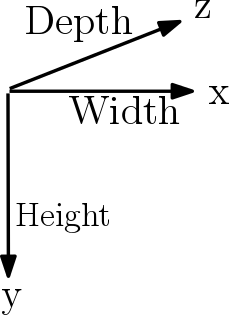
\includegraphics[width=\textwidth]{img/arrow3D}
    \caption{Dimensions represented.}
    \label{fig:3b}
  \end{subfigure}
  \caption{Three dimensional array representation.}
  \label{fig:3D}
\end{figure}

In the normal mutidimensional array synatx of C++, this will become, an array of arrays of arrays of ints.
See Listing~\ref{lst:3dexample}.
We transvers it using three nested loops, where the most outer one is the one indexed by the new dimension.

\begin{listing}[H]
  \inputminted[
    firstline=40, %If you omit this two fields, the whole file is pulled
    lastline=64
  ]{cpp}{src/ArrayDimensions.cpp}
  \caption{Three dimensional array example in C++}
  \label{lst:3dexample}
\end{listing}

For memory flatening, we will need a new version of functions $g$ and $h$, that depends in a new extra parameter: \mintinline{cpp}{DEPTH}.
In Listing~\ref{lst:functions3D}, we can see the new function $g$.

\begin{listing}[H]
  \inputminted[
    firstline=123, %If you omit this two fields, the whole file is pulled
    lastline=143
  ]{cpp}{src/FlatMemmory.cpp}
  \caption{New function $g$ to map real index into simulated 3D indices}
  \label{lst:functions3D}
\end{listing}

I will talk about the form of the function for the second result (the $y$ that represents the \mintinline{cpp}{j} index) in Section~\ref{sec:moreDim}.
Finally, for completenees; the new function $h$ is presented in Listing~\ref{lst:functions3D2}

\begin{listing}[H]
  \inputminted[
    firstline=145, %If you omit this two fields, the whole file is pulled
    lastline=163
  ]{cpp}{src/FlatMemmory.cpp}
  \caption{A new function $h$ to map simulated 3D indices into the real index, this is the inverse of $g$}
  \label{lst:functions3D2}
\end{listing}

\subsubsection{Generalizing to more dimensions}
\label{sec:moreDim}

In the case of two dimensions the calculation in function $g$ were simply the integer division and the modulo.
In the case of three dimensions we also have a modulo and a division (Altrought, the parameters change in the later one).
However, the interesting case is that of the middle value: it has both operations.

This is actually the general case.
Indeed, the correct transformation to get the simulated index of a given dimension, is as follows:
\begin{enumerate}
  \item Divide the real index by the size of the unit of all the previous dimensions.
  \item Take the result of the previous operation and  calculate his modulo with the maximum size of the given dimension.
\end{enumerate}

Let me present in Listing~\ref{lst:functions3D3} an alternative to the function $g$ showed in Listing~\ref{lst:functions3D} using the general appproach.

\begin{listing}[H]
  \inputminted[
    firstline=187, %If you omit this two fields, the whole file is pulled
    lastline=205
  ]{cpp}{src/FlatMemmory.cpp}
  \caption{Alternative $g$ function for 3D. Using the general form of the algorithm}
  \label{lst:functions3D3}
\end{listing}

Now, it becomes clear why in Listing~\ref{lst:functions3D} we did not need the full forms.
For the $x$ variable the previous dimension has size one, and we do not need to divide by one.
As for the last variable $z$, we know that \mintinline{cpp}{index} is striclly less than \mintinline{cpp}{WIDTH * HEIGHT * DEPTH}, and we divide it by \mintinline{cpp}{WIDTH * HEIGHT}, so it should be a number stricltly less than \mintinline{cpp}{DEPTH}, therefore we do not need to take the modulo.

Now that the the logic of the function $g$ is clear; we can also come up with a general rule for the inverse function $h$.

\begin{enumerate}
  \item For each dimension calculate a term.
        The term is the size of the unit in the previos dimension times the index in the current dimension.
  \item Accumulate (add) all the terms to calculate the real index.
\end{enumerate}

See Listing~\ref{lst:functions3D4} for the \emph{general rule} implementation.

\begin{listing}[H]
  \inputminted[
    firstline=166, %If you omit this two fields, the whole file is pulled
    lastline=185
  ]{cpp}{src/FlatMemmory.cpp}
  \caption{Alternative to function $h$ using the general rule}
  \label{lst:functions3D4}
\end{listing}

\section{Bit manipulation}

In this section I will explian some bit manipulation operations.
As it's common in most programing tasks and to avoid difficult cases: we will foucus on positive values for integer types.

Just to clarify the terms: \emph{bit} is a single binary digit, it can have only two values either 0 or 1.
A \emph{byte} is a group of bits that conforms the unit of the computer architecture.
Technically, a byte can have any size in bits.
However, in modern computers this is always 8.
That is why sometimes they call a byte an \emph{octet}.
For the following code samples you can assume the following constant to be in scope.

\begin{minted}{cpp}
const size_t BITS_PER_BYTE = 8U;
\end{minted}

Let me introduce, in Listing~\ref{lst:binHelpers}; two helper functions to debug and visulize such variables.
The first one: \mintinline{cpp}{bitSize} returns the size in bits of the variable and the second one: \mintinline{cpp}{bitStr} returns a string with the binary representation of a variable.

{\centering
\begin{minipage}{\linewidth}
  \begin{listing}[H]
  \inputminted[
  xleftmargin=1.5cm,  %without this option line number goes wrong
  %frame=lines,
  framesep=0.5cm,
  baselinestretch=1.2,
  fontsize=\footnotesize,
  linenos,
  firstline=76, %If you omit this two fields, the whole file is pulled
  lastline=86
  ]{cpp}{src/bitOperations.cpp}
  \caption{Helper functions to debug bit manipulations}
  \label{lst:binHelpers}
  \end{listing}
\end{minipage}
\par
}

Another important feature in C++ is that we can use binary (since standar C++14) and heaxadecimal literals:
\begin{minted}{cpp}
unsigned char aChar = 0b101010;
int anInt = 0xFF00FF08;
cout << "binary representation of aChar: " << binStr(aChar) << endl;
cout << "binary representation of anInt: " << binStr(anInt) << endl;
\end{minted}
The above code will print:
\begin{verbatim}
binary representation of aChar: 00101010
binary representation of anInt: 11111111000000001111111100001000
\end{verbatim} 

\subsection{Bit's operations}

The operations that work at bits level are the following:
\begin{itemize}
\item Shift to the left by $n$ bits. Performed with the operator \mintinline{cpp}{<<}.
\item Shift to the right by $n$ bits. Performed with the operator \mintinline{cpp}{>>}.

These binary operations take an integer value (in the left hand side) and an unsigned integer value (in the right hand side) and return the result of an integer value of the same size of the left operand created by shifting the bits of the left operand by the number of bits represented by the right operand.
The bits shifted out are discarded and in order to fill the spaces created by the shift, zeros are inserted.
Because of this, shifting to any side by the exact size in bits of the left operand is the same as setting the result to 0.
And of course, shifting to any side by 0, it's a null operation, the left operand it's returned without modification.
However, a quick warning note: Shifting to any side by a number greater than the size (in bits) of the left operand or by a negative number it is not defined.
See~\cite{INT34Cpp} for a more detailed explanation.
\item Bitwise \emph{AND} between two values of the same size.
      Performed with the operator \mintinline{cpp}{&}.
      Yes, it is the same as the \emph{dereference} operator.
      The distinctions is made due the former being a binary operator and the dereference one being a unary operator.
\item Bitwise \emph{OR} between two values of the same size.
      Performed with the operator \mintinline{cpp}{|}
\item Bitwise \emph{XOR} between two values of the same size.
      Also known as \emph{exclusive or}.
      Performed with the operator \mintinline{cpp}{^}

These operators are the expected equivalent to the ones defined in first order logic.
However, they operate bitwise; that is why they are different than the logical ones that are represented by double ampersand or double pipe.

\item Bitwise unary \emph{NOT}.
      Performed with the operator \mintinline{cpp}{~}
\end{itemize}

The code snippet in Listing~\ref{lst:bitShifting} shows a valid C++ sample of these operations:

{\centering
\begin{minipage}{\linewidth}
  \begin{listing}[H]
  \inputminted[
  xleftmargin=1.5cm,  %without this option line number goes wrong
  %frame=lines,
  framesep=0.5cm,
  baselinestretch=1.2,
  fontsize=\footnotesize,
  linenos,
  firstline=36, %If you omit this two fields, the whole file is pulled
  lastline=47
  ]{cpp}{src/bitOperations.cpp}
  \caption{Sample of bit shiting}
  \label{lst:bitShifting}
  \end{listing}
\end{minipage}
\par
}

Produces the following output:

\begin{verbatim}
a: 00101010 = 42
b: 01010000 = 80
c: 00000101 = 5
d: 00000000 = 0
e: 00000000 = 0
\end{verbatim} 

Another important thing to notice is that, \emph{as long as the shift leaves significant digits} (or else we \emph{underflow}); shifting values to the right is equivalent to divide by $2^n$ where $n$ is the number of bits shifted.
Similarly, shifting values to the left, \emph{as long as we do not discard a significant bit} (or else we \emph{overflow}); is equivalent to multiply by $2^n$, where $n$ is the number of bits shifted.
Note also that \mintinline{cpp}{unsigned} types cannot underflow.

In the above sample $2^3 = 8$.
Therfore: $c = 42 / 8 = 5$ (remember it's an integer division).
And $b = 42 \cdot 8 = 336$, but it resulted in an overflow, since the maximun value for an $8$ bit variable is $2^8 = 256$.


Listing~\ref{lst:bitwiseOp} present a sample usage of the bitwise logical operations:

{\centering
\begin{minipage}{\linewidth}
  \begin{listing}[H]
  \inputminted[
  xleftmargin=1.5cm,  %without this option line number goes wrong
  %frame=lines,
  framesep=0.5cm,
  baselinestretch=1.2,
  fontsize=\footnotesize,
  linenos,
  firstline=50, %If you omit this two fields, the whole file is pulled
  lastline=71
  ]{cpp}{src/bitOperations.cpp}
  \caption{Bitwise operations sample}
  \label{lst:bitwiseOp}
  \end{listing}
\end{minipage}
\par
}

And produces the following result:

\begin{verbatim}
c = a & b
a: 10101101
b: 11100110
c: 10100100
d = a | b
a: 10101101
b: 11100110
d: 11101111
e = a ^ b
a: 10101101
b: 11100110
e: 01001011
f = ~a
a: 10101101
f: 01010010
\end{verbatim}

\subsection{Bit manipulations}

In order to do bit manipulations, we need to be able to refer to a specific bit.
The bits on a variable are refered by a position.
The first position, is the rightmost bit; which is refered as $0$, and positions continue to increment by one to the left until the last bit.
Look at the Figure~\ref{fig:bitPos}.
Therefore, in an $8$ bit size variable positions are in $\{ 0, 1, \ldots, 6, 7 \}$ and in a $32$ bit variable are in $\{ 0, 1, \ldots, 30, 31 \}$.

\begin{figure}[htb]
  \centering
  \begin{subfigure}[b]{0.35\textwidth}
    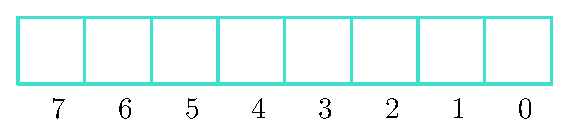
\includegraphics[width=\textwidth]{img/bitPositions}
    \caption{Bit positions for an $8$ bit variable.}
    \label{fig:bitPosa}
  \end{subfigure}
  \hspace*{1cm}
  \begin{subfigure}[b]{0.35\textwidth}
    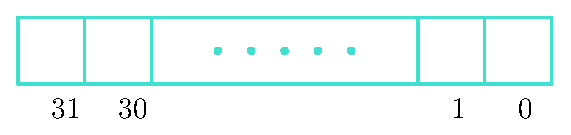
\includegraphics[width=\textwidth]{img/bitPositions2}
    \caption{Bit positions for a $32$ bit variable.}
    \label{fig:bitPosb}
  \end{subfigure}
  \caption{Positions of the bits in a variable.}
  \label{fig:bitPos}
\end{figure}

Extra note: \emph{endianism does not matter for bit manipulations}.
The lenguaje (in this case C++) abstract this for you.
Endianism only matters when you are reading or writing to the filesystem.
So, for the purposes of this explanation: all machines are big endian.

There are four important operations for bit manipulation:
\begin{description}
\item[Set] Put in an specific bit to the value of $1$.
\item[Clear] Put in an specific bit to the value of $0$.
             Also known as \emph{reset} or \emph{unset}.
\item[Toggle] Change the value of a specific bit.
              In other words: if the bit is $1$ set it to $0$, else set it to $1$.
\item[Query] This operation results in a boolean value.
             If an specif bit is $1$ return \mintinline{cpp}{true}, else return \mintinline{cpp}{false}.
\end{description}

In order to implement the bit manipulation we have to use the bit operations in combination with what is called a \emph{mask}.
A mask is another variable; of the same size of the one we want to manipulate, that only contain ones in the places we want to manipulate.
Well, technically a mask could be of any size, but the explanation get easier if you imagine them of the same size.

As an example, lets construct an $8$ bit mask for manipulating the bit at position $3$.
\begin{itemize}
 \item We start with the value of $1$, in binary representation: $00000001$.
 \item Now, we shift to the left by $n$ bits. Where $n$ is the desired position.
 \item In other words to construct the mask we could do: \mintinline{cpp}{1 << 3}.
 \item The mask is: $00001000$
\end{itemize}

Now that we have the mask, it becomes obvious that we can use it to operate it with the variable to manipulate the bit corresponding to the mask.
For example, to set the bit at position $2$ of a variable, we make a bitwise $OR$ between the corresponding mask and the variable.
The result is a new value that has the value of $1$ at the place where the mask is pointing, and it's equall to the original variable in all the other positions.

\begin{minted}{cpp}
unsigned char a = 0b00101010;
unsigned char mask = 1 << 2; // Mask for bit at postion 2
unsigned char r = a | mask;
cout << "a: " << binStr(a) << endl;
cout << "m: " << binStr(mask) << endl;
cout << "r: " << binStr(r) << endl;
\end{minted}
The previous code snippet will print:
\begin{verbatim}
a: 00101010
m: 00000100
r: 00101110
\end{verbatim}

The rest of the bit manipulations can be perfomed in a similar way by combining the bitwise operations and the mask.
The long code sample in Listing~\ref{lst:bitManip} shows explicitlly how to archive the bit manipulations.

{\centering
\begin{minipage}{\linewidth}
  \begin{listing}[H]
  \inputminted[
  xleftmargin=1.5cm,  %without this option line number goes wrong
  %frame=lines,
  framesep=0.5cm,
  baselinestretch=1.2,
  fontsize=\footnotesize,
  linenos,
  firstline=26, %If you omit this two fields, the whole file is pulled
  lastline=59
  ]{cpp}{src/bitManipulation.cpp}
  \caption{Bit manipulation presented in a long explicit way}
  \label{lst:bitManip}
  \end{listing}
\end{minipage}
\par
}

The output of the code in Listing~\ref{lst:bitManip} is:
\begin{verbatim}
Original value
a: 00101010
Create a mask for the bit at position 2
m: 00000100
Variable to show the reult
r: 00000000
Setting a bit: r = a | mask
a: 00101010
m: 00000100
r: 00101110
Clearing a bit: r = a & (~mask)
a: 00101010
m: 00000100
~m:11111011
r: 00101010
Toggling a bit: r = a ^ mask
a: 00101010
m: 00000100
r: 00101110
Query a bit: q = ((a & mask) != 0)
The bit is false
\end{verbatim}

Finally, the above sample in Listing~\ref{lst:bitManip}, was written in a long form that prefers clarity on explanation rather than brevity in the code.
Indeed, the most common (and compact) way to perform bit manipulations does not use a temporal storage for the mask.
And operates in place: using the same variable as operand and output.
The Listing~\ref{lst:bitManip2} shows a sample of the most common usage.

{\centering
\begin{minipage}{\linewidth}
  \begin{listing}[H]
  \inputminted[
  xleftmargin=1.5cm,  %without this option line number goes wrong
  %frame=lines,
  framesep=0.5cm,
  baselinestretch=1.2,
  fontsize=\footnotesize,
  linenos,
  firstline=24, %If you omit this two fields, the whole file is pulled
  lastline=51
  ]{cpp}{src/bitManipulation2.cpp}
  \caption{Most common way of making bit manipulations}
  \label{lst:bitManip2}
  \end{listing}
\end{minipage}
\par
}

Which produces the following output:
\begin{verbatim}
10101011
Setting the bit at position 2
10101111
Setting the bit at position 0 (nothing happens since was already set)
10101111
Clearing the bit at position 3
10100111
Clearing the bit at position 6 (nothing happens since was already clear)
10100111
Toggling the bit at position 2
10100011
The bit at position 4 is unset
10100011
The bit at position 5 is set
10100011  
\end{verbatim}

\subsection{Manipulating groups of bits}

The general case is to manipulate a group of bits, and it's done in the same way as individual bits.
Remember, that we said that a mask contain ones in the places where we want to manipulate and zeros anywhere else.
Then, to manipulate several bits at once, we just need a more general mask.

This is particlary usefull when we operate on bigger integer types, like $32$ or $64$ bit sizes.
The usual way to construct these masks is to use hexadecimal literals.
In hexadecimal each digit represent $4$ bits.
For example, to create a mask that operates on bits $6$, $7$ and $8$ of a $32$ bit variable. 

\begin{minted}{cpp}
unsigned int mask = 0x000001c0;
cout << "m: " << binStr(mask) << endl;
\end{minted}

Will print:
\begin{verbatim}
m: 00000000000000000000000111000000
\end{verbatim}

Typically an \mintinline{cpp}{unsigned char} has $8$ bits size and an \mintinline{cpp}{unsigned int} has $32$ bits size.
However, if you want to be sure (and not really in conventions), you can also use types with explicit size since C++11, like \mintinline{cpp}{uint8_t} and \mintinline{cpp}{uint32_t}.
They just require the header \mintinline{cpp}{#include <cstdint>}. 
The hexadecimal representation it's particularly usefull since a literal of the form $0xXX$, where the $X$ represents an hexadecimal digit; can create a mask for an \mintinline{cpp}{unsigned char}.
And a literal in the form $0xXXXXXXXX$ can do it for an \mintinline{cpp}{unsigned int}.

\section{Analytic Geometry}

I will use the convention from~\cite{Buss2003}.
We use lower case names in normal font to represent scalars: $s$, $t$, $v$.
Bolt font with lower case names to represent vectors: $\mathbf{a}$, $\mathbf{b}$, $\mathbf{p}$.
Upper case names in bold face to represent set of points in the space: $\mathbf{L}$, $\mathbf{R}$ (like lines or rays).
Finally, upper case names in normal font to represent matrices: $P$, $V$, $M$.

The vectors are column vectors. In other words:
$$ \mathbf{v} = \begin{pmatrix}
  x \\ 
  y \\
  z
 \end{pmatrix} $$

Then we can use syntax like: $A \mathbf{x} = \mathbf{b}$.
To make the reading easier, in case I will need to specify a vector inside a paragraph I will use $\mathbf{v} = \langle x, y, z \rangle$

In the notation, we do not make any distinction between vectors and points, therefore the text always give context to clarify this. 

\subsection{Line, ray and segment}

In most CG applications, we use two \emph{different} points; let's call them $\mathbf{a}$ and $\mathbf{b}$ (with $\mathbf{a} \neq \mathbf{b}$) to specify a line: $\mathbf{L}$. 

However, in analytic geometry we prefer a parametric equation for the line: $\mathbf{L}(t)$.
We use a point $\mathbf{p}$, a directional vector $\mathbf{v}$ and a scalar $t$ as parameter : $\mathbf{L}(t) = \mathbf{p} + t \mathbf{v}$, with $t \in (-\infty, \infty)$.

To transform between this two representations we do: $\mathbf{v} = \mathbf{b} -\mathbf{a}$. And, then the line is: 

\begin{equation}
\mathbf{L}(s) = \mathbf{a} + s (\mathbf{b} -\mathbf{a}) = \mathbf{a} + s \mathbf{v} 
\label{eq:line}
\end{equation}
, with $s \in (-\infty, \infty)$. 

Note that the order of $\mathbf{a}$ and $\mathbf{b}$ is relevent, because of the way we define $\mathbf{v}$: it points from $\mathbf{a}$ to $\mathbf{b}$.
Also note that $\mathbf{v}$ is not necesarlly a unit vector. 

\begin{figure}[htb]
  \centering
  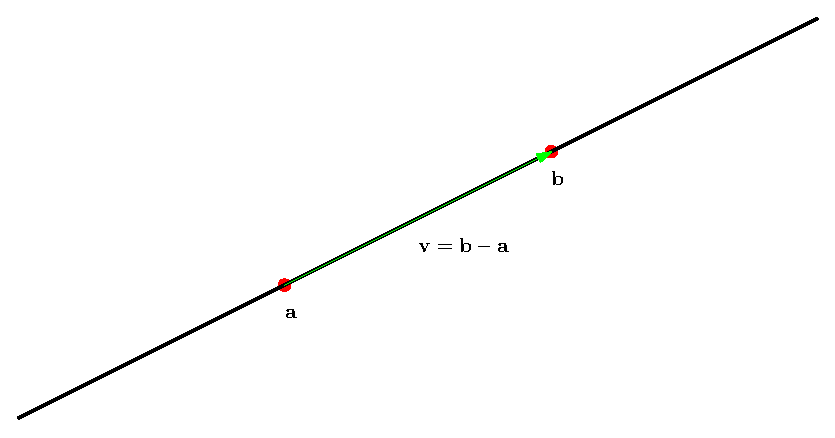
\includegraphics[width=0.85\textwidth]{img/line}
  \caption{Line identified by two points. See Equation~\ref{eq:line} }
  \label{fig:line}
\end{figure}

The Figure~\ref{fig:line} shows the line from Equation~\ref{eq:line} indentified by the points $\mathbf{a}$ and $\mathbf{b}$.
On these conditions; we can give continuos values to the parameter $s$ in the Equation~\ref{eq:line}, to obtain points on the line $\mathbf{L}$.
Particulary, if we let $s = 0$ we get the point $\mathbf{a}$ and if we let $s = 1$ we get  
$\mathbf{b}$.
Moreover, any value $0 \leq s \leq 1$ will get us a point $\mathbf{p}$ inside the line segment $\overline{\mathbf{a} \mathbf{b}}$.
Any value $s > 1$ will get a $\mathbf{p} \in \mathbf{L}$, $\mathbf{p} \notin \overline{\mathbf{a} \mathbf{b}}$ that is closer to $\mathbf{b}$ than it is to to $\mathbf{a}$.
Conversely, any $s < 0$ will get a $\mathbf{p} \in \mathbf{L}$, $\mathbf{p} \notin \overline{\mathbf{a} \mathbf{b}}$ that is closer to $\mathbf{a}$ than it is to $\mathbf{b}$.

We can use this last observations to identify segments and rays.
A \emph{ray} from $\mathbf{a}$ in the direction of $\mathbf{b}$ is the one that has Equation~\ref{eq:line}, with the constrain that the parameter must be $s \geq 0$.
The line \emph{segment} from $\mathbf{a}$ to $\mathbf{b}$, denoted by $\overline{\mathbf{a} \mathbf{b}}$, is the one that also follows Equation~\ref{eq:line}, with the constrain that   $0 \leq s \leq 1$.

\subsection{Point to line distance}

Given a line $\mathbf{L}$ and a point $\mathbf{p}$, we want to identify the distant $d$ from $\mathbf{p}$ to $\mathbf{L}$.
It's clear that if $\mathbf{p} \in \mathbf{L}$, then $d = 0$.
Now, if $\mathbf{p} \notin \mathbf{L}$, we want the distant between $\mathbf{p}$ and a certain point $\mathbf{q}$, such that $\mathbf{q} \in \mathbf{L}$ and $d(\mathbf{q}, \mathbf{p})$ is the minimal to all other points in $\mathbf{L}$.

\begin{figure}[htb]
  \centering
  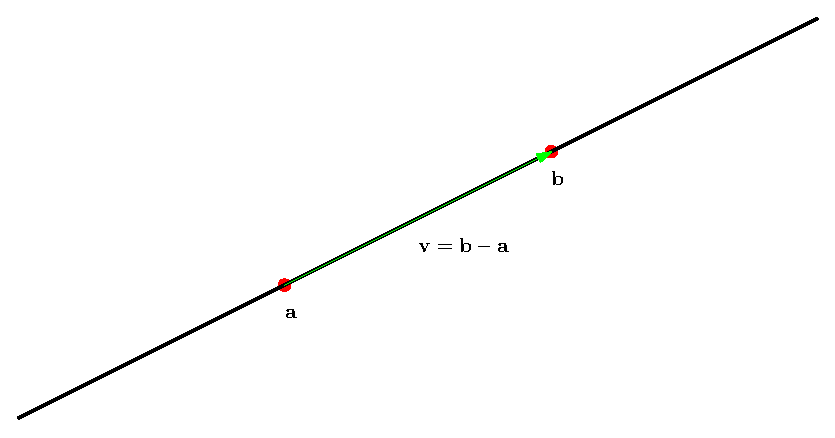
\includegraphics[width=0.85\textwidth]{img/line}
  \caption{Distance $d(\mathbf{p}, \mathbf{L})$ between a point $\mathbf{p}$ and a line $\mathbf{L}$}
  \label{fig:point2line}
\end{figure}

In other words we want the minimal distance from $\mathbf{p}$ to $\mathbf{L}$.
The Figure~\ref{fig:point2line} depicts this situation.
If we start sliding a point on $\mathbf{L}$ (strating lets say at $\mathbf{p}$) and evaluating the distance beween that point and $\mathbf{p}$, we can see that the distance start getting smaller as we come close to $\mathbf{p}$, get his minimal value when we are right bellow $\mathbf{q}$ and then increases again. 
Indeed, the distance we are looking is between $\mathbf{p}$ and the point $\mathbf{q}$ that is in the intesection between the lines $\mathbf{L}$ and $\mathbf{M}$
Where $\mathbf{M}$ is the line perpendicular to $\mathbf{L}$ that toches $\mathbf{p}$. 

Before proceding I put a quick reminder of the formula to calculate the projection of a vector $\mathbf{x}$ into another vector $\mathbf{y}$.

\begin{equation}
\proj_{\mathbf{y}}\mathbf{x} = \dfrac{(\mathbf{x} \cdot \mathbf{y})}{|\mathbf{y}|} \dfrac{\mathbf{y}}{|\mathbf{y}|} = \dfrac{(\mathbf{x} \cdot \mathbf{y})}{|\mathbf{y}|^2}\mathbf{y}
\label{eq:proj}
\end{equation}

In order to calculate the distance we use the Equation~\ref{eq:proj} to find the corresponding parametric value $s_q$ for $\mathbf{q}$ on $\mathbf{L}$: 
\begin{equation}
s_q = \dfrac{(\mathbf{p} - \mathbf{a}) \cdot (\mathbf{b} - \mathbf{a})}{|\mathbf{b} - \mathbf{a}|^2}
\label{eq:scalarq}
\end{equation}
Then the point is:
\begin{equation}
\mathbf{q} = \mathbf{a} + s_q (\mathbf{b} -\mathbf{a})
\label{eq:pointq}
\end{equation}
And finally, the distance is $d(\mathbf{p}, \mathbf{L}) = d(\mathbf{p}, \mathbf{q})$.
\subsubsection{Point to segment distance}

Another common derived problem is to find the distance of a point $\mathbf{p}$ to a segment $\overline{\mathbf{a}\mathbf{b}}$.
See Figure~\ref{fig:point2line}, we see the distance of the different points depend on how are they placed with respect of the segment.
For the point $\mathbf{p}_1$ the distance to the segment is the distance $d(\mathbf{p}_1, \mathbf{a})$, for the point $\mathbf{p}_2$ the distance is $d(\mathbf{p}_2, \mathbf{b})$ and for the point $\mathbf{p}_3$ the distance is actually the distance $d(\mathbf{p}_3, \mathbf{L})$ where $\mathbf{L}$ is the line defined by $\mathbf{a}$ and $\mathbf{b}$.

The observations at the end of Section and Section give us a nice Algorithm to find this distance.

{\centering
\begin{minipage}{\linewidth}
  \begin{algorithm}[H]
    \caption{Distance between a point $\mathbf{p}$ and a line segment $\overline{\mathbf{a}\mathbf{b})}$}
    \label{alg:euclid}
    \begin{algorithmic}[1] % The number tells where the line numbering should start 0 for no number
      \Procedure{DistancePoint2Segment}{$\mathbf{a},\mathbf{b},\mathbf{p}$} \Comment{$\mathbf{a}$ and $\mathbf{b}$ are vectors and $\mathbf{p}$ is a point all of the same dimension}
        \If{$\mathbf{a} = \mathbf{b}$} \Comment{There is no line it's just a point}
          \State \textbf{return} $d(\mathbf{a},\mathbf{p})$
        \EndIf
        \State $s \gets \frac{(\mathbf{p} - \mathbf{a}) \cdot (\mathbf{b} - \mathbf{a})}{|\mathbf{b} - \mathbf{a}|^2}$ \Comment{Use Equation~\ref{eq:scalarq} to get parametric value of $\mathbf{q}$}
        \If{$s < 0$} \Comment{$\mathbf{p}$ is closer to $\mathbf{a}$ than to $\overline{\mathbf{a}\mathbf{b}}$}
          \State $r \gets d(\mathbf{a},\mathbf{p})$
         \ElsIf{$s > 1$} \Comment{$\mathbf{p}$ is closer to $\mathbf{b}$ than to $\overline{\mathbf{a}\mathbf{b}}$}
          \State $r \gets d(\mathbf{b},\mathbf{p})$
        \Else \Comment{$\mathbf{p}$ is over $\overline{\mathbf{a}\mathbf{b}}$}
          \State $\mathbf{q} \gets \mathbf{a} + s (\mathbf{b} - \mathbf{a})$ \Comment{Calculate $\mathbf{q}$}
          \State $r \gets d(\mathbf{q},\mathbf{p})$
        \EndIf
        \State \textbf{return} $r$ \Comment{Distance is stored in $r$}
      \EndProcedure
    \end{algorithmic}
  \end{algorithm}
\end{minipage}
\par
}

\subsection{Ray to segment intersection}

Another common problem is to test if a ray $\mathbf{R}$ intersects a line segment $\mathbf{S}$.
The ray its defined by a point of origin $\mathbf{o}$ and a directional vector $\mathbf{u}$.
As usual, the segment is defined by his two end points $\mathbf{a}$ and $\mathbf{b}$.

In the scenario described above, the ray is $\mathbf{R}(s) = \mathbf{o} + s \mathbf{v}$ with $s \geq 1$ and the segment is $\mathbf{S}(t) = \mathbf{a} + t (\mathbf{b} - \mathbf{a})$ with $0 \leq t \leq 1$.
If $\mathbf{R}(s)$ intersects $\overline{\mathbf{a}\mathbf{b}}$, then $\mathbf{R}(s) = \mathbf{S}(t)$ for some values of $\mathbf{s}$ and $\mathbf{t}$.

\begin{align*}
\mathbf{a} + t (\mathbf{b} - \mathbf{a}) &= \mathbf{o} + s \mathbf{v} \\
\mathbf{a} - \mathbf{o} &= s \mathbf{v} + t (\mathbf{a} - \mathbf{b})
\end{align*}

\subsection{Belonging test on simple polygons}


\section{Graphics Pipeline}

\subsection{Common pipeline}
\label{sec:commPipe}

As is defined in OpenGL 4.6, it is the most common version of the pipeline.  If you are interview for a graphics position chances are that they refer to this pipeline. None of the  optional shader stages are present. See the Section~\ref{sec:compPipe} for the complete pipeline.

\begin{itemize}
 \item Vertex specification.
 \begin{itemize}
  \item It is started with a drawing command and a properly set shader program.
  \item Retrive vertex arrays from CPU as per VAO specification.
  \begin{itemize}
   \item Vertex array objects (Vertex data)
   \item Vertex index buffer (Primitive assemble instructions)
  \end{itemize}
  \item Retrive shader uniforms.
  \item Fill vertex attributes.
 \end{itemize}

 \item Vertex shader.
 \begin{itemize}
  \item User defined programable stage.
  \item It is mandatory.
  \item Execution appears to be parallel for each vertex. The user has no knowledge of order execution.
  \item Map input and output in a 1:1 way. There most be exactlly one output per input. Because of this it can be cached. A vertex with the same input must have the same output, therefore can be skipped the second time.
  \item If you want to draw something, it must output normalize device coordinates. Also known as clip coordinates. 
  \begin{itemize}
   \item A vector of four components. The first three must be in $[-1, 1]$
   \item It represent the vertex position in homogenous coordinates in the viewing volume.
   \item It is typically archived by multpliying the input position by the Projection, View and Model matrices: $P V M\mathbf{x}$
  \end{itemize}

 \end{itemize}

 \item Vertex post processing.
 \begin{itemize}
  \item Transformation feedback can optionally happen here. Output of the primitives are written into buffer objects.
  \item Clipping: All primitives that lies in the boundary are broken into smaller primitives that are inside the viewing volume.
  \item Perspective division. The vertex position is divided by the $w$ coordinate.
  \item Viewport transformation. The vertex is mapped into (possiblly more than one) discrete screen coordinates according to the output framebuffer.
 \end{itemize}

 \item Primitive assembly.
 \begin{itemize}
  \item All vertex are assamble into primitives inside the viewing volume. Typically triangles.
  \item Face culling can optionally happen. Due the winding order of the triangles and the fact that you are in normalize device coordinates. You can take the dot product between the normal of the rendring plane ($\mathbf{k}$) and the normal of the triagle: $(\mathbf{p}_1 - \mathbf{p}_0) \times (\mathbf{p}_2 - \mathbf{p}_0)$ order matters. And you know which face is facing the camera (back or front).
 \end{itemize}

 \item Rasterization.
 \begin{itemize}
  \item Primitive are rasterized in the order thay were given.
  \item The result is a fragment, that is the set of properties used to compute the final color of a pixel.
  \item If multisampling is enable a fragment is created per sample (and the state include coverage info)
 \end{itemize}

 \item Fragment shader.
 \begin{itemize}
  \item User defined programable optional stage.
  \item Execution appears to be parallel for each sample. The user has no knowledge of order execution.
  \item You have access to all the user defined attributes per sample and his positon in the ouput frambuffer.
  \item You can discard a fragment or sample.
  \item The ouput (if you want to draw) must be one color per each output frambuffer expected. Plus depth values and stencil values. 
  \item If you do not supply one, the depth and stencil values are still output to the frambuffers, and the color buffer content it's not defined.
 \end{itemize}

 \item Per sample operations.
 \begin{itemize}
  \item A series of tests that the fragment goes to see if it will become a pixel in the output frambuffer. Most of them are optional.
  \item Pixel ownership test. If the pixel is not owned by the OpenGL context this test fails. It is the only non optional test. If you draw to a framebuffer object, this test alway pases.
  \item Siccssor test: optional, fails if the pixel lies ourside a user defined rectangle of the screen.
  \item Stencil test: optional, when its enable, the pixel performs a user defined operation with the contents of the stencil buffer. And optionally writes to the buffer. If fail the pixel is discarded.
  \item Depth test: optional, the pixel depth value is compared with the one in the buffer if is less, then overrides the buffer and passes, if it is not then it is discarded.
  \item Blending: this is not a test, but an operation that all the pixel perform to store his content into the output frambuffer. It is user configurable and typically uses alpha value to perform transparency.
  \item Write to the output framebuffers. An optional last masking of certain channels can happen (maybe you disable writting to the depth).
 \end{itemize}

\end{itemize}


\subsection{Complete pipeline}
\label{sec:compPipe}

It is the same as the previous section but with the optional programable stages active.
The two stages are the Tesselation stage and the Geometry stage.

\begin{itemize}
 \item Vertex specification.
 \item Vertex shader.
 \item Tesselation shader.
 \begin{itemize}
  \item Optional, programable user defined stage.
  \item It is divided in two:
  \begin{itemize}
   \item Tesselation control shader. Determines the amount of tesselation and the geometry of a primitive. It is optional even if the tesselation stage is active.
   \item Tesselation evaluation shader. Determines the values of the primitive attributes after the tesselation happens. It must be present if the tesselation stage is active
  \end{itemize}
 \end{itemize}
 \item Geometry shader
 \begin{itemize}
  \item It recieves the primitives used for drawing.
  \item Can optionally change the primitive type, number and modify vertex attributes.
  \item It must output the vertex position in normalize device coordinates (Hence replacing the positions from the Vertex shader).
 \end{itemize}
 \item Vertex post processing.
 \item Primitive assembly.
 \item Rasterization.
 \item Fragment shader.
 \item Per sample operations.
\end{itemize}

\subsection{Texture pipeline}
\label{sec:textPipe}
%Add these books to the reference table even if we do not cite them explicitly
\nocite{Gottschling2015}
\nocite{Laakmann2015}
%Add the references
\printbibliography
\end{document}
